% =====================================================================
%  IEEE two-column conference paper (IEEEtran). Compile with pdfLaTeX.
%  Overleaf: Menu -> Compiler: pdfLaTeX. Main document: main.tex
%  All numbers below come from the experiment outputs (nhanes_study/).
%  Lines marked "% TODO" need your team's input (names, affiliations).
% =====================================================================
\documentclass[conference]{IEEEtran}
\IEEEoverridecommandlockouts

\usepackage{cite}
\usepackage{amsmath,amssymb}
\usepackage{graphicx}
\usepackage{booktabs}
\usepackage{array}
\usepackage{xcolor}
\usepackage[hidelinks]{hyperref}
\graphicspath{{figures/}}

\begin{document}

\title{Classical Machine Learning vs. Deep Learning for Cardiovascular Disease Classification: An Explainable AI Study Using NHANES Data}

% TODO: replace with your real names, departments and emails
\author{
\IEEEauthorblockN{Author One}
\IEEEauthorblockA{\textit{Department of Computer Science} \\
\textit{University Name}\\
City, Country \\
email@university.edu}
\and
\IEEEauthorblockN{Author Two}
\IEEEauthorblockA{\textit{Department of Computer Science} \\
\textit{University Name}\\
City, Country \\
email@university.edu}
}

\maketitle

% ---------------------------------------------------------------------
\begin{abstract}
Cardiovascular disease (CVD) classification from routinely collected clinical data offers a setting to compare the accuracy and interpretability of machine-learning methods. Using four cycles (2011--2018) of the National Health and Nutrition Examination Survey (NHANES; $n = 21{,}552$ adults, 2{,}369 with self-reported CVD), we compared Logistic Regression, Random Forest, Support Vector Machine and XGBoost with a multilayer perceptron (MLP) on 20 harmonized demographic, clinical and laboratory features. All models achieved similar discrimination on a held-out test set (ROC-AUC 0.839--0.848); XGBoost performed best (0.848, 95\% CI 0.829--0.863), and the MLP (0.842) did not differ significantly from any classical model (DeLong $p \geq 0.064$). All models were well calibrated (ECE $\leq 0.018$), and under temporal validation on 2017--2018 data every model reached an AUC of 0.837--0.839. The MLP required the longest tuning time and about 170 times the training time of Logistic Regression. SHAP analysis identified age as the most influential feature for every model, and feature rankings were broadly concordant (Kendall's $W = 0.75$), but agreement clustered by model family: tree ensembles agreed closely with each other ($\rho = 0.94$), as did smooth-boundary models (SVM--MLP $\rho = 0.89$). Feature-group ablation confirmed the dominance of demographic variables. Inverse attributions for cholesterol were traced to post-diagnosis treatment, underscoring that attributions reflect predictive association, not causation. For structured clinical survey data, deep learning provided no measurable advantage over classical approaches.
\end{abstract}

\begin{IEEEkeywords}
Cardiovascular disease, classical machine learning, deep learning, NHANES, explainable artificial intelligence, SHAP
\end{IEEEkeywords}

% ---------------------------------------------------------------------
\section{Introduction}
Cardiovascular diseases (CVDs) are a major public health concern associated with demographic, physiological, biochemical, and behavioral factors~\cite{tsao2023,roth2020}. Clinical variables such as age, blood pressure, cholesterol, glucose concentration, and body mass index provide valuable information for investigating cardiovascular health and underpin established risk scores~\cite{dagostino2008,goff2014}. However, relationships among these variables can be nonlinear and interdependent, motivating the application of data-driven predictive methods.

Classical machine learning algorithms, including Logistic Regression, Support Vector Machines, Random Forests, and gradient-boosted decision trees, are widely applicable to structured clinical data. These methods offer different trade-offs between interpretability, computational efficiency, and the ability to capture nonlinear relationships. Deep learning models, particularly multilayer perceptrons, can learn complex feature interactions but may require careful regularization and sufficient training data. Their greater complexity does not necessarily guarantee superior performance on tabular health datasets~\cite{christodoulou2019,grinsztajn2022,shwartzziv2022}.

Model evaluation in clinical applications should extend beyond predictive accuracy. Identifying which features influence predictions, determining whether their contributions remain stable across algorithms, and assessing probability calibration are important for evaluating model reliability~\cite{vancalster2019}. Explainable artificial intelligence techniques, including SHapley Additive exPlanations (SHAP)~\cite{lundberg2017}, provide a framework for examining feature contributions. However, model attribution indicates predictive influence rather than causation~\cite{rudin2019}.

The National Health and Nutrition Examination Survey (NHANES), conducted by the United States Centers for Disease Control and Prevention, combines health interviews, physical examinations, and laboratory measurements~\cite{nhanes}. Integrating four survey periods provides an opportunity to compare predictive models using population-level clinical data. Such integration requires consistent variable definitions, appropriate handling of missing data, and consideration of survey design and changes in data collection~\cite{johnson2013}.

This study compares classical machine learning models with a multilayer perceptron for cardiovascular disease classification using harmonized NHANES data. It evaluates predictive performance, calibration, and computational efficiency while examining clinical feature contributions through SHAP and feature-ablation experiments. The study further investigates whether different model families identify consistent influential features, providing a comparative assessment of predictive effectiveness and interpretability on structured clinical data.

% ---------------------------------------------------------------------
\section{Related Work}
% TODO: review and edit. Facts about each study are taken from the cited papers.
Machine learning for CVD risk has been studied in large cohorts. Weng \textit{et al.}~\cite{weng2017} compared logistic regression, random forests, gradient boosting and neural networks against the ACC/AHA risk score in UK primary-care records, and Ambale-Venkatesh \textit{et al.}~\cite{ambale2017} applied random survival forests to the Multi-Ethnic Study of Atherosclerosis. Alaa \textit{et al.}~\cite{alaa2019} showed that an automated machine-learning ensemble outperformed the Framingham score in 423{,}604 UK Biobank participants. A meta-analysis by Krittanawong \textit{et al.}~\cite{krittanawong2020} reported high pooled discrimination but substantial heterogeneity across outcomes and datasets.

Several studies have used NHANES. Dinh \textit{et al.}~\cite{dinh2019} compared logistic regression, SVM, random forest, gradient boosting and an ensemble for diabetes and CVD. Martin-Morales \textit{et al.}~\cite{martinmorales2023} predicted CVD mortality from health and nutrition variables and used SHAP for interpretation, and Ahiduzzaman and Hasan~\cite{ahiduzzaman2025} compared five classical models with SHAP and LIME on NHANES 2017--2023. None of these studies compared classical models with a tuned neural network under the same pipeline, and none measured whether attributions agree across model families or remain stable across refits.

Evidence from broader benchmarks suggests that machine learning rarely outperforms logistic regression in clinical prediction~\cite{christodoulou2019} and that tree ensembles often match or exceed deep learning on tabular data~\cite{grinsztajn2022,shwartzziv2022}. Explanation methods can also disagree with one another~\cite{krishna2024}. This study addresses these gaps by comparing five model families on identical data splits, with calibration, temporal validation, and cross-model and within-model SHAP stability.

% ---------------------------------------------------------------------
\section{Dataset and Methodology}

\subsection{Data and Cohort}
We combined four NHANES cycles (2011--2012, 2013--2014, 2015--2016, 2017--2018)~\cite{nhanes}. The 2019--2020 cycle was excluded because data collection was interrupted by COVID-19. The analytic cohort comprised adults aged $\geq 20$ years who completed the mobile examination and had a determinable outcome ($n = 21{,}552$; 2{,}369 cases). Prevalence was 11.0\% unweighted and 8.9\% survey-weighted, using the examination weight divided by four as recommended for combined cycles~\cite{johnson2013}.

\subsection{Outcome}
CVD was defined as a self-reported physician diagnosis of congestive heart failure, coronary heart disease, angina, heart attack or stroke (items MCQ160B--F). Participants answering ``no'' to all five were controls; those with refused, unknown or missing answers were excluded ($n = 94$).

\subsection{Features and Preprocessing}
Twenty features were harmonized across cycles: age, sex, race/ethnicity (four indicators), income-to-poverty ratio, education, systolic and diastolic blood pressure (mean of up to three readings), pulse rate, BMI, waist circumference, total and HDL cholesterol, HbA1c, serum creatinine, uric acid, smoking status and diagnosed diabetes. Medication variables were excluded because treatment frequently follows a CVD diagnosis and would leak the label. Missingness was at most 9.8\%. Median imputation and standardization were fitted inside each model pipeline on training folds only.

\subsection{Models and Training}
Data were split 80/20 with stratification (training $n = 17{,}241$; test $n = 4{,}311$). Hyperparameters were tuned by five-fold stratified cross-validation on the training set to maximize ROC-AUC. We trained L2-regularized Logistic Regression (LR), Random Forest (RF)~\cite{breiman2001}, an RBF-kernel SVM~\cite{cortes1995} with Platt-scaled probabilities~\cite{platt1999}, XGBoost (XGB)~\cite{chen2016} tuned by 40-iteration random search~\cite{bergstra2012}, and an MLP. The MLP used Linear--BatchNorm--ReLU--Dropout blocks~\cite{ioffe2015,srivastava2014}, the AdamW optimizer~\cite{loshchilov2019} and early stopping on a 15\% validation split; 60 configurations were searched, and the selected network (64--32 hidden units, dropout 0.5) had 3{,}649 parameters. Models were implemented in scikit-learn~\cite{pedregosa2011}, XGBoost and PyTorch~\cite{paszke2019}. Each model's decision threshold maximized F1 on out-of-fold training predictions.

\subsection{Evaluation}
On the test set we report ROC-AUC with 1{,}000-sample bootstrap confidence intervals, PR-AUC~\cite{saito2015}, precision, recall, F1, Brier score~\cite{brier1950}, expected calibration error (ECE)~\cite{naeini2015} and calibration slope~\cite{vancalster2019}. Paired AUC differences were tested with DeLong's method~\cite{delong1988,sun2014}. Robustness was assessed over five random splits, by temporal validation (train 2011--2016, test 2017--2018), and with survey-weighted AUC.

\subsection{Explainability and Stability}
To make attributions comparable, the same model-agnostic permutation SHAP estimator~\cite{lundberg2017} was applied to every model's predicted probability (300 test rows, 50 background rows). Its rankings agreed with exact TreeSHAP~\cite{lundberg2020} for XGBoost ($\rho = 0.989$). Cross-model agreement was measured with pairwise Spearman correlation of mean $|\text{SHAP}|$ and Kendall's $W$~\cite{kendall1939}; within-model stability used five bootstrap refits. Feature-group ablation removed one of eight groups at a time and averaged the AUC change over five splits.

% ---------------------------------------------------------------------
\section{Results and Discussion}

\subsection{Predictive Performance}
Table~\ref{tab:perf} and Fig.~\ref{fig:roc} summarize test performance. All five models fell within 0.009 AUC. XGBoost was significantly better than LR ($p = 0.005$), RF ($p < 0.001$) and SVM ($p = 0.002$), but not than the MLP ($p = 0.064$); the MLP did not differ significantly from any classical model. All models were well calibrated; the MLP had the largest ECE and a slope below one.

\begin{table*}[t]
\caption{Test-Set Performance ($n = 4{,}311$; 474 CVD Cases)}
\label{tab:perf}
\centering
\setlength{\tabcolsep}{4pt}
\resizebox{\textwidth}{!}{%
\begin{tabular}{lccccccccc}
\toprule
Model & CV AUC (SD) & Test AUC [95\% CI] & PR-AUC & Precision & Recall & F1 & Brier & ECE & DeLong $p$ vs MLP \\
\midrule
Logistic Regression & 0.846 (0.009) & 0.839 [0.821--0.855] & 0.392 & 0.383 & 0.561 & 0.455 & 0.080 & 0.010 & 0.321 \\
Random Forest       & 0.847 (0.003) & 0.839 [0.821--0.856] & 0.407 & 0.361 & 0.586 & 0.447 & 0.080 & 0.010 & 0.460 \\
SVM (RBF)           & 0.849 (0.007) & 0.839 [0.821--0.854] & 0.396 & 0.362 & 0.584 & 0.447 & 0.080 & 0.007 & 0.274 \\
\textbf{XGBoost}    & 0.850 (0.005) & \textbf{0.848 [0.829--0.863]} & \textbf{0.418} & 0.373 & 0.572 & 0.451 & \textbf{0.078} & 0.009 & 0.064 \\
MLP                 & 0.849 (0.007) & 0.842 [0.825--0.858] & 0.398 & 0.390 & 0.523 & 0.447 & 0.080 & 0.018 & -- \\
\bottomrule
\end{tabular}}
\end{table*}

\begin{figure*}[t]
\centering
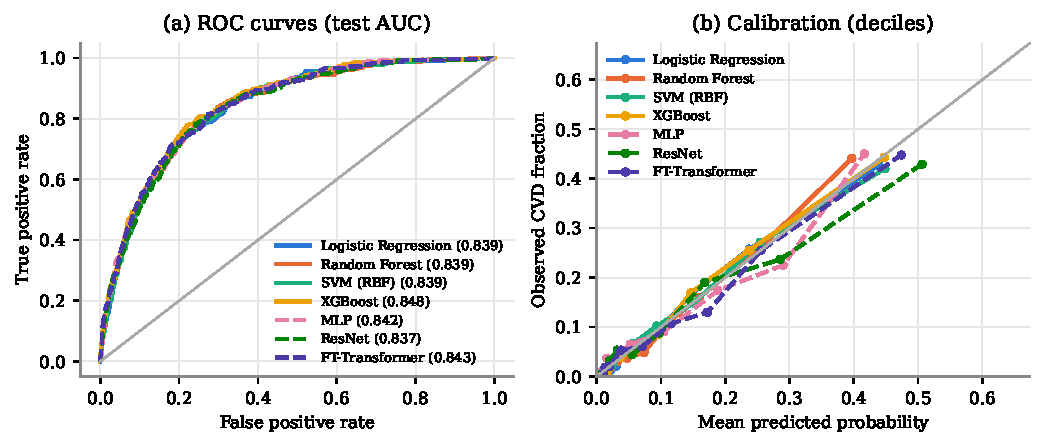
\includegraphics[width=0.85\textwidth]{fig1_roc_calibration.pdf}
\caption{(a) ROC curves on the test set (AUC in legend). (b) Calibration by decile of predicted risk.}
\label{fig:roc}
\end{figure*}

\subsection{Robustness and Efficiency}
Across five random splits the models differed by less than one standard deviation, and under temporal validation all converged to an AUC of 0.837--0.839 (Table~\ref{tab:robust}). The MLP was the most expensive to tune and about 170 times slower to fit than LR; the SVM was the slowest at inference and explanation.

\begin{table}[t]
\caption{Robustness and Computational Cost}
\label{tab:robust}
\centering
\setlength{\tabcolsep}{3pt}
\resizebox{\columnwidth}{!}{%
\begin{tabular}{lccccc}
\toprule
 & LR & RF & SVM & XGB & MLP \\
\midrule
AUC, 5 splits (mean)   & 0.842 & 0.841 & 0.843 & 0.846 & 0.844 \\
\quad SD               & 0.002 & 0.004 & 0.003 & 0.004 & 0.003 \\
Temporal AUC           & 0.838 & 0.837 & 0.838 & 0.838 & 0.839 \\
Weighted test AUC      & 0.852 & 0.851 & 0.853 & 0.862 & 0.855 \\
\midrule
Tuning time (s)        & 5     & 271   & 224   & 49    & 352 \\
Fit time (s)           & 0.05  & 1.49  & 47.4  & 0.62  & 9.04 \\
Inference (ms/1k)      & 1.1   & 24.8  & 828   & 2.9   & 1.2 \\
SHAP, 300 rows (s)     & 10    & 120   & 1615  & 10    & 5 \\
\bottomrule
\end{tabular}}
\end{table}

\subsection{Feature Attributions and Stability}
Age was the most important feature for every model (Fig.~\ref{fig:shap}). Overall agreement was high (Kendall's $W = 0.746$), but it clustered by model family (Table~\ref{tab:stab}): RF and XGB agreed closely ($\rho = 0.941$), as did SVM and MLP ($\rho = 0.886$), while cross-family pairs ranged from 0.47 to 0.66. Tree models had the most stable full rankings across bootstrap refits, whereas LR, SVM and MLP kept a more stable top five.

\begin{figure}[t]
\centering
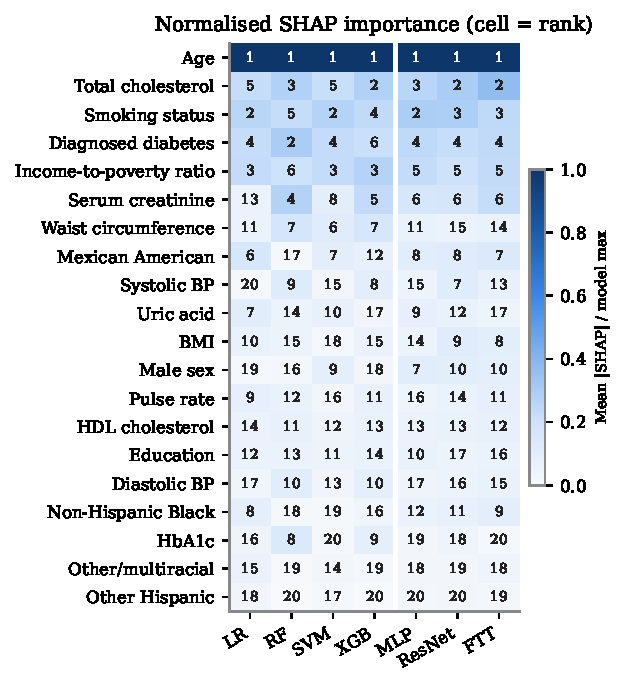
\includegraphics[width=0.82\columnwidth]{fig2_shap_importance_heatmap.pdf}
\caption{Mean $|$SHAP$|$ per model, scaled to each model's top feature. Cell numbers are within-model ranks.}
\label{fig:shap}
\end{figure}

\begin{table}[t]
\caption{SHAP Ranking Agreement (Spearman $\rho$) and Within-Model Stability}
\label{tab:stab}
\centering
\setlength{\tabcolsep}{3.5pt}
\resizebox{\columnwidth}{!}{%
\begin{tabular}{lccccc}
\toprule
 & LR & RF & SVM & XGB & MLP \\
\midrule
RF  & 0.474 &       &       &       & \\
SVM & 0.656 & 0.653 &       &       & \\
XGB & 0.553 & \textbf{0.941} & 0.663 &   & \\
MLP & 0.743 & 0.629 & \textbf{0.886} & 0.633 & \\
\midrule
Bootstrap $\rho$      & 0.846 & 0.973 & 0.732 & 0.921 & 0.805 \\
Top-5 Jaccard         & 0.867 & 0.767 & 1.000 & 0.733 & 1.000 \\
\bottomrule
\end{tabular}}
\end{table}

\subsection{Feature-Group Ablation}
Removing demographic features caused the largest loss for every model (Fig.~\ref{fig:abl}), largest for LR ($-0.063$ AUC). Lipid, glycaemic, socioeconomic, renal and smoking groups each cost 0.002--0.007, while anthropometric and blood-pressure groups contributed almost nothing.

\begin{figure}[t]
\centering
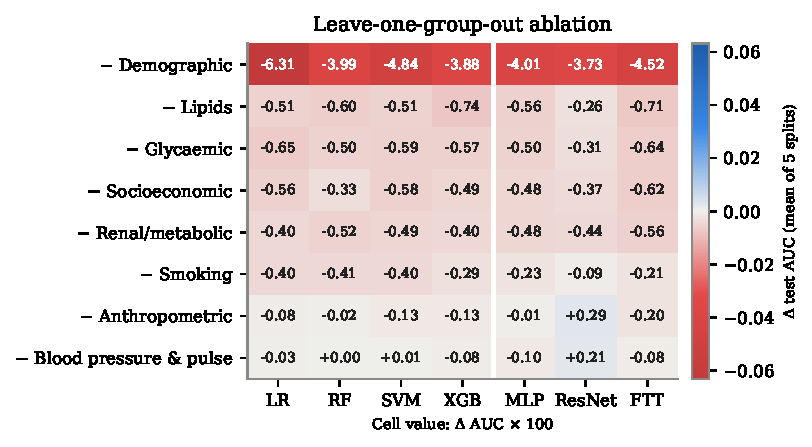
\includegraphics[width=0.95\columnwidth]{fig4_ablation.pdf}
\caption{Change in test AUC ($\times 100$) when each feature group is removed, averaged over five splits.}
\label{fig:abl}
\end{figure}

\subsection{Discussion}
Deep learning gave no measurable advantage, consistent with benchmarks on tabular data~\cite{grinsztajn2022,shwartzziv2022} and clinical prediction~\cite{christodoulou2019}. LR came within 0.009 AUC of the best model at a fraction of the cost. Similar accuracy did not imply similar explanations: tree ensembles and smooth-boundary models distribute credit differently among correlated features, so attributions from a single model give an incomplete picture~\cite{krishna2024,hooker2021}.

Higher total cholesterol lowered predicted CVD probability in every model, and blood pressure added almost no information. Both reflect treatment after diagnosis: survey-weighted statin use was 58.0\% among cases versus 14.2\% among controls, and antihypertensive use was 62.8\% versus 20.1\%. Because the outcome is prevalent, self-reported CVD measured cross-sectionally, the models partly learn markers of diagnosis and treatment rather than risk of developing CVD, and attributions describe association only. Further limitations are recall bias in self-report, age top-coded at 80, and the use of survey weights for descriptive analysis rather than model training. Future reporting should follow TRIPOD+AI~\cite{collins2024}.

% ---------------------------------------------------------------------
\section{Conclusion and Future Work}
On harmonized NHANES 2011--2018 data, four classical models and an MLP achieved nearly identical discrimination and calibration for CVD classification, and the MLP offered no significant gain at a substantially higher computational cost. SHAP identified age as the dominant feature for all models, but attribution agreement depended on model family. Future work should use incident outcomes from linked mortality data, include treatment status explicitly, and incorporate the survey design into model training.

% ---------------------------------------------------------------------
\bibliographystyle{IEEEtran}
\bibliography{refs}

\end{document}
